\documentclass[aps,rmp, twocolumn]{revtex4}
%\documentclass[a4paper,10pt]{scrartcl}
%\documentclass[aps,rmp,twocolumn]{revtex4}

\usepackage[utf8]{inputenc}
\usepackage{amsmath,graphicx}
\usepackage{color}
%\usepackage{cite}

\newcommand{\Richard}[1]{{\color{red}Richard: #1}}
\newcommand{\LH}{\mathcal{L}}
\newcommand{\rvec}{\mathbf{r}}


\begin{document}
\title{When to trust phylogeographic inferences?}
\author{Richard Neher}
\date{\today}
\begin{abstract}
    Sometimes.
\end{abstract}

\maketitle
As organisms replicate, they also disperse in space, potentially exploring new habitats.
The reconstruction of ancestral locations and past migrations from sampling locations of extant individuals, typically in combination with genome sequence information to infer the phylogeny, is known as phylogeography.
Phylogeographic methods are implemented in popular evolutionary analysis software such as BEAST \citep{pybus_unifying_2012}.
The underlying model of dispersal is typically diffusive, that is the probability of sampling a descendant at position $\rvec_c$ after time $t$ when the parent was at position $\rvec_p$ is given by
\begin{equation}
    P(\rvec_c| \rvec_p, t) = \frac{1}{4\pi D t}e^{\frac{|r_c - r_p|^2}{4Dt}}
\end{equation}
where $D$ is a diffusion constant with dimensions $\mathrm{length}^2/\mathrm{time}$, and we have assumed a two-dimensional space.
Each branch in the phylogeny is decorated with such a diffusive propagator.
Such a diffusive process is the simplest and most natural choice in absence of directed motion or long range migration.
It is also mathematically convenient as unknown ancestral locations can be integrated in closed form and the marginal distribution of each position can be calculated exactly for a fixed tree along with the likelihood. 
The total likelihood of the configuration is then assumed to be the product of the spatial likelihood and the phylogenetic likelihood, i.e. tree topology and branching rates of the tree are assumed to be independent of the spatial process.
However, these two interact in important ways, for example when a population expands into an uninhabited fertile habitat or a disease spreads in a susceptible population.

In a typically Bayesian phylogeographic inference problem as discussed in \citet{pybus_unifying_2012}, the input data are typically viral genome sequences as well as their sampling times and sampling locations.
Software like BEAST will then sample the posterior distribution of the phylogenetic tree topology, the sampling times and locations of ancestral nodes in the tree, and model parameters like the diffusion constant $D$ and the evolutionary rate $\mu$.
Results can be estimates of the ancestral location of a particular groups of samples, or summary statistics of the dispersal process.
Popular summaries include empirical estimates of the diffusion constant  \citep{pybus_unifying_2012} and a so-called \emph{dispersal velocity} \citep{dellicour_using_2017}. These are calculated from the estimated displacements along branch $i$ with parent $p_i$ given by $d_i = |\rvec_{p_i} - \rvec_{i}|$ and the elapsed time $\Delta t_i$ as
\begin{equation}
    D_w = \frac{\sum_{i\in B}d_i^2}{4\sum_{i\in B} \Delta t_i} \quad \mathrm{and}  \quad v_w = \frac{\sum_{i\in B} d_i}{\sum_{i\in B} \Delta t_i}
\end{equation}
where $B$ is the set of all branches of the tree.
Effectively $D_w$ divides the sum of all observed squared displacements by the total time elapsed on the tree to obtain and estimate of $D$.
It is known as the `weighted' estimate of the diffusion constant.
The weighted dispersal velocity estimate compares the sum of absolute values of observed displacements to the total time, which has dimensions of a velocity.
Alternative formulations use the mean of fractions $D_b = |B|^{-1} \sum_{i\in B}d_i^2/4t_i$ or $v_b = |B|^{-1} \sum_{i\in B}d_i/t_i$ instead of the ratio of sums. \
We refer to these here as `by branch' estimates. 
The latter tend to be dominated by short branches and thus noisier. 


The purpose of this note is to explore how sensitive phylogeographic inferences are to model assumptions and what quantities can be robustly estimated.
My focus here is only on the ability and robustness to estimate dispersal parameter and ancestral locations and I will assume perfect knowledge of the tree and the sampling locations.
So no tree-sampling will be necessary.
To explore qualitatively different behaviors, I will consider Kingman and Yule tree ensembles. Kingman trees are the classical neutral model of a constant size population, while Yule trees capture features of growing populations (see Fig.~\ref{fig:illustration_tree}).

\begin{figure*}[tb]
    \includegraphics*[width=0.7\textwidth]{figures/illustration_tree.pdf}
    \caption{\label{fig:illustration_tree}{\bf Illustration Yule and Kingman trees and the spatial location of the tips.}
    The total tree length of Yule trees is proportional to the number of tips $n$ and the time to the MRCA is $\log(n)$.
    Kingman trees have a total tree length that is proportional to $\log(n)$ and are characterized by rapid merging close to the present. }
\end{figure*}


Fig.~\ref{fig:D_and_v} shows empirical estimates of diffusion constants and velocity as defined above from simulated data using freely diffusing locations along Kingman trees.
The diffusion constant $D$ can be estimated robustly from these data and are compatible with the diffusion constant used to simulate the data $D=1$.
Values of $v_w$ and $v_b$, however, depend strongly on the sample size. 
That the velocity estimates are ill-defined is not surprising: By changing the sample size, the average length of branches changes. Diffusion along each branch results in a displacement of $d_i \sim \sqrt{4Dt_i}$ such that a quantity that depends on $\Delta d_i / t_i \sim 1/t_i^{1/2}$ will change with the time $t_i$ that elapsed along the branch.
With more samples in the tree, the average branch length decreases and the velocity estimates increase. 
This expected scaling $\sim \sqrt{n}$ is indicated by the dashed line in Fig.~\ref{fig:D_and_v}.
For Yule trees, the average branch length is independent of the number of samples and the velocity estimates are more stable. 
But estimates for $v_w$ and $v_b$ are not consistent with each other and their numerical values have no interpretation within the model.

In either case, estimates of $v_w$ or $v_b$ are not meaningful. 
The underlying model is diffusive and has no parameters that individually or combined would have dimensions of a velocity. 
There is no ground truth to compare the estimates to and $v_w$ and $v_b$ are just descriptive summaries of spatial spread with unclear interpretation.


\begin{figure}[tb]
    \includegraphics*[width=0.48\textwidth]{figures/kingman_dispersal.pdf}
    \caption{\label{fig:D_and_v}{\bf Empirical summary statistics of $D$ and ``dispersal velocity'' for different sample sizes.}
    While diffusion constant $D$ (equal to 1 in this example) can be robustly estimated from simulation data of the underlying model, the dispersal rate $v_w$ (weighted) and $v_b$ (by branch) are not well-defined quantities. Their numerical value depends strongly on sample size and there is no ground truth to compare to. The expected scaling $\sim \sqrt{n}$ of $v$ estimates is indicated by the dashed line.}
\end{figure}

\section*{How does density regulation affect estimates phylogeographic estimates?}
Phylogeographic inference typically assumes that the spatial diffusion process is independent of the branching pattern of the tree and ignores coupling between the two. 
Such a coupling could, for example, arise when growth rates depend on local population density, and it has been known for a long time that ignoring such coupling leads to very unrealistic population densities \citep{felsenstein_pain_1975}.
If one simulates a diffusive spatial process in a square of length $L$ with periodic boundary conditions, the population density shows strong fluctuations whenever the diffusion constant $D<L^2/T_c$, where $T_c$ is the coalescent times scale of the population (see Fig.~\ref{fig:heterogeneity}).
In a well-mixed neutral model, $T_c$ is equal to the population size $N$.  

For $D<L^2/2T_c$, the time to the most recent common ancestor $T_{MRCA}$ is too small for the population to spread evenly in the habitat.
This is illustrated in Fig.~\ref{fig:heterogeneity}A that shows the population distribution across the habitat for $D=0.1L^2/T_c$. 
The population distribution is patchy with large uninhabited areas.
This heterogeneity increases substantially for even lower $D$, when the population is essentially a cloud of width $\sqrt{4DT_c}\ll L$.
Fig.~\ref{fig:heterogeneity}B quantifies this heterogeneity as the standard deviation of population density in two-dimensional bins of different size  relative to the expectation in the case of a spatially well-mixed population. 

\begin{figure*}[tb]
    \includegraphics*[width=\textwidth]{figures/heterogeneity_free_diffusion.pdf}
    \caption[short]{\label{fig:heterogeneity}{\bf Population density variation in free diffusion models.}
    When spatial motion is independent of population density and coalesce is sufficiently rapid, the realized population density fluctuates strongly across the habitat. The left panel shows the population density for the case $D = 0.1 L^2/N$ in linear bins of size $L/20$. The right panels shows the standard deviation of the population density for different bin sizes as a function of the diffusion coefficient. For $D>L^2/N$, the heterogeneity approaches the expected value in the well mixed limit. }
\end{figure*}

Biological populations spread into areas that support them and will quickly populate fertile areas that are below their carrying capacity.
A simple model for the population density $\phi(x,t)$ would be 
\begin{equation}
    \label{eq:FKPP}
    \frac{\partial \phi(x,t)}{\partial t} = D\frac{\partial^2 \phi(x,t)}{\partial x^2} + \alpha \phi(x,t)(1-\phi(x,t)/\phi_0)
\end{equation}
where $\phi_0$ is the carrying capacity and $\alpha$ is the population growth rate at zero density.
This model has a stable fixed point at $\phi=\phi_0$.
In a static environment, we thus expect the population density to settle at a constant density $\phi_0$ and density fluctuations will decay with rate $\alpha$. 

While dependence of growth (and thus tree structure) on density is a key component of real-world population dynamics, it is difficult to implemented in phylogeographic inference frameworks.
It is, however, fairly straightforward to include density dependence in forward simulations and these simulations can be used to investigate the effect of such coupling between growth and spatial location on phylogeographic inferences.
We calculate the population density using a Gaussian kernel with interaction radius $r$
\begin{equation}
    \phi(\rvec) = \sum_{i\in N} \frac{e^{-|\rvec_i - \rvec|^2/2r^2}}{N\sqrt{2\pi r^2}}
\end{equation}
where the sum is over all individuals $i$ in the population of size $N$.

As soon as the interaction radius $r$ is much smaller than the habitat size, this density regulation leads to a more homogeneous population density, see Fig.~\ref{fig:density_reg}.
Diffusion constants estimated from the population remain accurate with moderate overestimation of small diffusion constants.
But with decreasing diffusion, the population fragments into smaller than smaller subpopulations that don't interact or coalesce.
This manifests in an increasing time to the MRCA, see Fig.~\ref{fig:density_reg}.
Spatial location and the coalescence process are thus strongly coupled, though this coupling manifests itself in population structure rather than estimates of the diffusion coefficients.
In such a spatially structured population, estimates of historical populations sizes (e.g.~skyline estimates) will be strongly affected. 

\begin{figure*}
    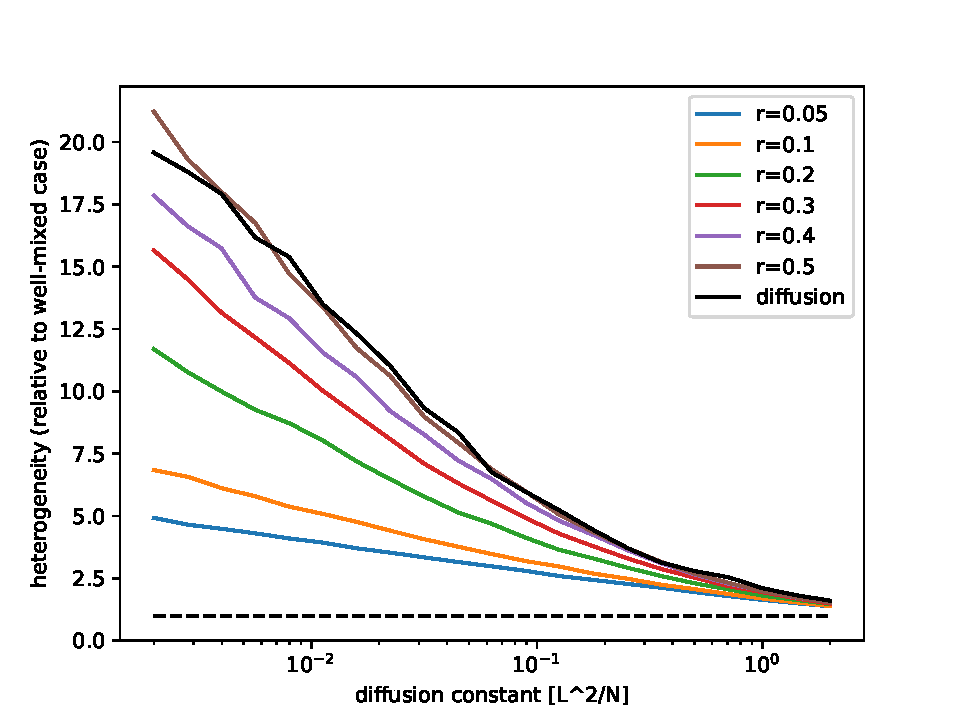
\includegraphics[width=0.48\textwidth]{figures/density_reg_heterogeneity.pdf}
    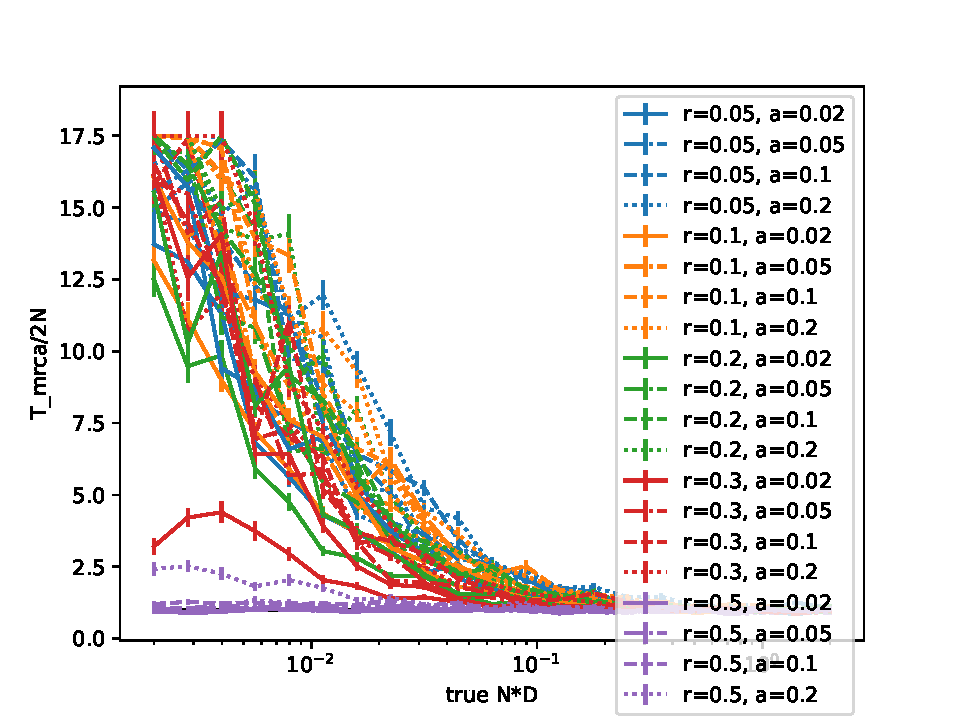
\includegraphics[width=0.48\textwidth]{figures/density_reg_tmrca.pdf}
    \caption{\label{fig:density_reg} {\bf Density regulation reduces fluctuations in density regulation, but results in population fragmentation at low diffusion constants.} The left panel shows population heterogeneity measured using bins of linear dimension $L/5$ for $\alpha =0.05$ for different values of the interaction radius $r$. For $r\ll L$, density fluctuations are strongly suppressed. At the same time, the time to the most recent common ancestor increases dramatically, indicating that the population fragments in subpopulations that don't interact.}
\end{figure*}

As discussed above, a static carrying capacity in an equilibrium population has limited effects on estimates of ancestral locations and diffusion coefficients. 
In reality, carrying capacities vary through time. 
Such variation happens on all time scales, ranging from environmental changes over millennia to seasonal fluctuations. 
The circulation of seasonal influenza viruses, for example, varies by many orders of magnitude between summer and winter in temperate climates.
Fluctuations in carrying capacity mean that populations not just spread because individuals move, but also because populations grow in regions where the population density is below the carrying capacity.
In such situations, the accuracy and interpretation of phylogeographic inferences are unclear. 

A simple model of the interplay between growth and spatial spread is again given by the Fisher-KPP equation (Eq.~\ref{eq:FKPP}) above. 
This equation admits solutions with a traveling front, that the population ``invades'' the empty territory with velocity $v_{FKPP} = 2\sqrt{D \alpha}$ \citep{fisher_wave_1937,KPP1937,hallatschek_life_2010}.
Note that the model itself does not have an explicit parameter that has dimensions of a velocity.
The speed at which the population invades space is given as compound of diffusion and accelerated growth in regions of low density and only grows like the square root of diffusion constant.

To explore such the result of such changing habitats on phylogeographic inferences, we simulated a habitat with a Gaussian carrying capacity that moves at a constant velocity $v$ along the $x$-axis (Fig.~\ref{fig:traveling_wave}). 
When varying the microscopic dispersal parameter $D$ and the velocity of the carrying capacity $v$, I observe diverse behavior with often dramatically overestimated $\hat{D}$. These behaviors are explained comparing the speed $v_{FKPP}$ at which the population can invade new territory with the external speed $v$, the ratio of which is used to plot the simulation data in Fig.~\ref{fig:traveling_wave}. 
For $v_{FKPP} \ll v$, the population cannot keep up with the moving carrying capacity and is saved from extinction only because selection is soft.
In this regime, the estimated velocity of lineages is below $v$ and both the estimated $v$ and $D$ increase with $v_{FKPP}$. 
Once $v\sim v_{FKPP}$, the estimated lineage velocity coincides with $v_{FKPP}$, while the estimated $D$ peaks at values orders of magnitude above the true value. 
For larger $v_{FKPP}$, the estimated velocity is stable for some time, before increasing again with $v_{FKKP}$ is a sampling dependent manner. 
At larger $v_{FKPP}$, $D$ is eventually underestimates.

In this extreme example of a population dragged along by a moving carrying capacity, estimates of dispersal rates are meaningless, and estimates of velocities are only compatible with the speed of the shifting habitat in a narrow range when the habitat speed matches the FKPP velocity.
Similarly, estimates of ancestral locations are biased to the current position of the habitat. 

Less extreme spatio-temporal dynamics of the habitat results in less extreme biases, but still illustrate that caution is required when interpreting phylogeographic inferences in environment that might change between the present and the $T_{MRCA}$ of the population.  
I simulated two additional scenarios: one habitat that expands and contracts to a core region periodically, and one that oscillates back and forth between two regions with a homogeneous intermediate state.

\begin{figure}
    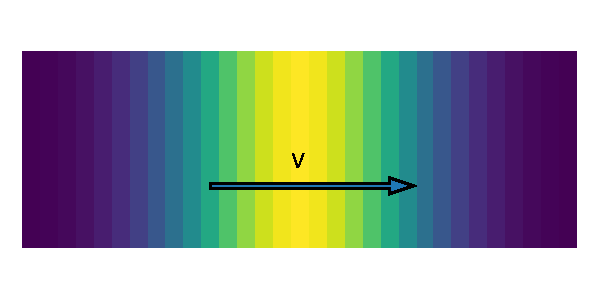
\includegraphics[width=0.48\textwidth]{figures/traveling_wave}
    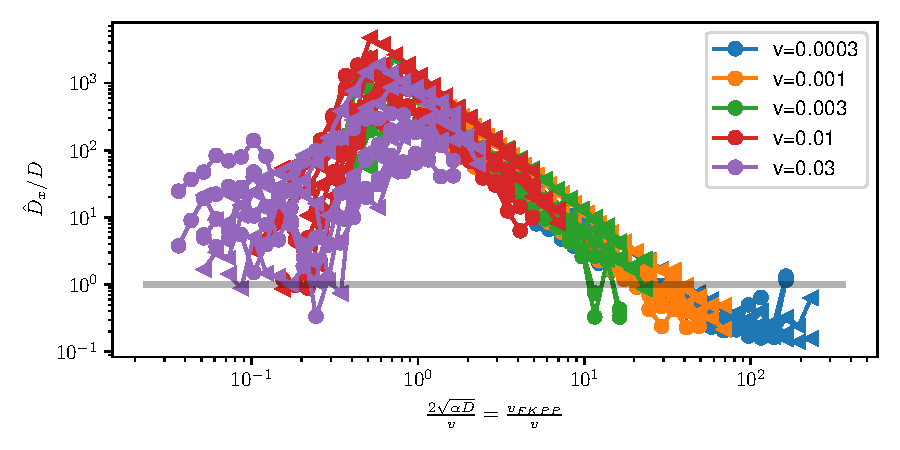
\includegraphics[width=0.48\textwidth]{figures/waves_D}
    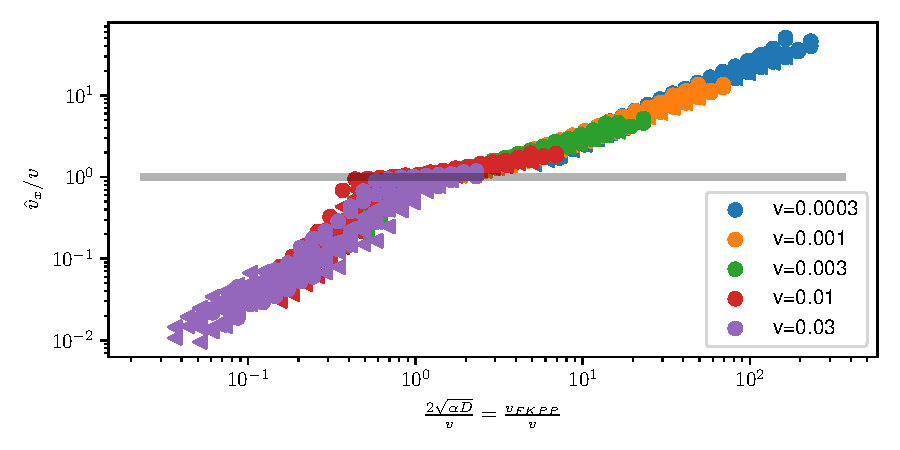
\includegraphics[width=0.48\textwidth]{figures/waves_v}
    \caption{\label{fig:traveling_wave} {\bf Phylogeographic estimates in rapidly changing environments.} Panel A shows an illustration of the simulated set-up: a carrying capacity with a Gaussian profile with $\sigma=0.5$ that moves along the $x$-axis with velocity $v$ on a patch with $L_x=3$, $L_y=1$, and periodic boundary conditions.
    Panels B\&C show estimates of diffusion coefficients and velocities, relative to their true values, as a function of the ratio of the FKPP velocity to the external velocity $v$. }
\end{figure}

\begin{itemize}
    \item periodic seasaws and other patters
    \item can we trust ancestral location inferences? with true D, with estimated D? significant biases?
    \item can we say something general? coalescence time versus diffusion time across the habitat, habitat changes vs fkpp speed
    \item typical FKPP speed: $D=km^2/day$, $\alpha = 0.2/day$. $v_{FKPP} = 2\sqrt{D\alpha} = km/day$.
\end{itemize} 

\section*{Discussion}


\bibliography{bib}


\end{document}


The above example assumed a habitat that is constant over times comparable to the time to the most recent common ancestor of the population.
If instead the habitat shifts on shorter time scales, the population has to move and such population movement will skew estimates of dispersal.
We simulated such changing habitats by assuming the carrying capacity of the habitat varies periodically in time and space
\begin{equation}
    \phi_0(\rvec, t) = N\left(1 + \sin(2\pi (r_x/L_x + t/T)\cos(2\pi (r_y/L_y + t/2T))) \right)
\end{equation}
This results in moving peaks and troughs in carrying capacity (and thus population density) as illustrated in

\begin{figure}
    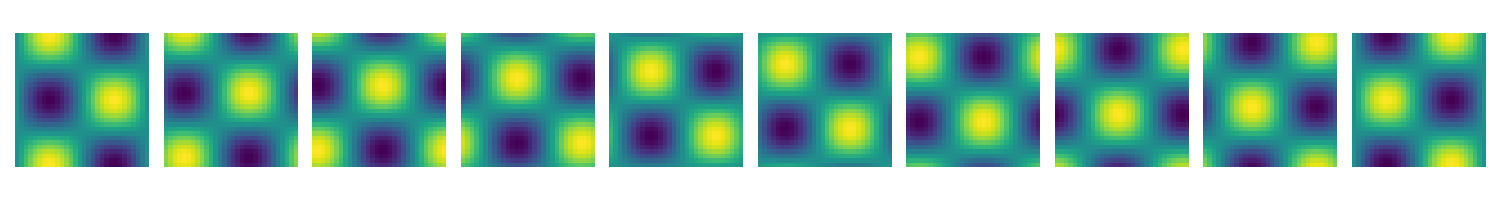
\includegraphics[width=\textwidth]{figures/habitats.png}
    \caption{\label{fig:moving_habitats}}
\end{figure}
